\documentclass[tikz,border=8pt]{standalone}
\usetikzlibrary{arrows.meta,positioning}

\begin{document}
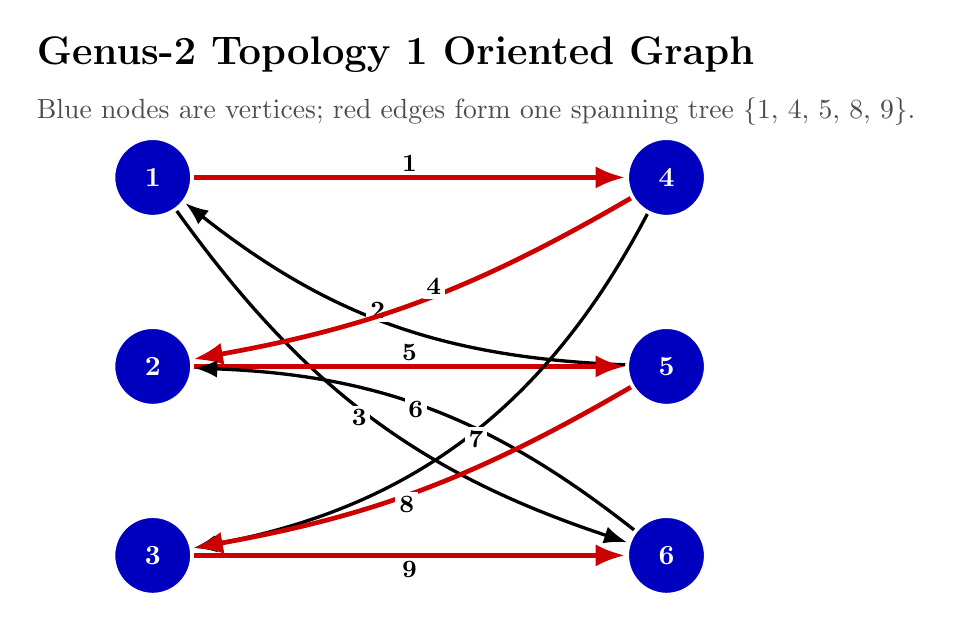
\begin{tikzpicture}[
  x=2.9cm,
  y=2.4cm,
  >=Latex,
  vertex/.style={circle, draw=white, line width=1.4pt, fill=blue!75!black, minimum size=10mm, inner sep=0pt, text=white, font=\bfseries},
  edge/.style={->, line width=1.2pt, draw=black},
  treeedge/.style={->, line width=1.7pt, draw=red!80!black},
  elabel/.style={fill=white, inner sep=1.4pt, font=\bfseries\small},
]

\node[anchor=west, font=\bfseries\Large, text=black] at (-0.55, 2.65) {Genus-2 Topology 1 Oriented Graph};
\node[anchor=west, font=\normalsize, text=black!70] at (-0.55, 2.35) {Blue nodes are vertices; red edges form one spanning tree \{1, 4, 5, 8, 9\}.};

\node[vertex] (v1) at (0,2) {1};
\node[vertex] (v2) at (0,1) {2};
\node[vertex] (v3) at (0,0) {3};
\node[vertex] (v4) at (2.25,2) {4};
\node[vertex] (v5) at (2.25,1) {5};
\node[vertex] (v6) at (2.25,0) {6};

\draw[treeedge] (v1) to node[elabel, above] {1} (v4);
\draw[edge] (v5) to[bend left=18] node[elabel, above left] {2} (v1);
\draw[edge] (v1) to[bend right=18] node[elabel, left] {3} (v6);
\draw[treeedge] (v4) to[bend left=10] node[elabel, above right] {4} (v2);
\draw[treeedge] (v2) to node[elabel, above] {5} (v5);
\draw[edge] (v6) to[bend right=18] node[elabel, left] {6} (v2);
\draw[edge] (v4) to[bend left=26] node[elabel, right] {7} (v3);
\draw[treeedge] (v5) to[bend left=10] node[elabel, below left] {8} (v3);
\draw[treeedge] (v3) to node[elabel, below] {9} (v6);

\end{tikzpicture}
\end{document}
